\chapter{实现与测试}

\section{实现平台与环境}
我们在\emph{gem5}模拟器上实现了MMT的原型,\emph{gem5}是一个多指令集的全系统模拟器,它可以模拟不同的指令集的(X86, ARM, RISCV, MIPS, SPARC等),不同的CPU模型:单周期,多周期,顺序执行,乱序执行,多发射等,不同的内存层次架构:
无缓存,L1缓存,L2缓存,L2缓存,以及指定每一级缓存的大小,集合,几路缓存等配置参数。同时gem5还对内存做了全模拟,实现了经典的内存模型以及ruby的内存模型。在模拟性能方面,gem5可以使用精确时间的模拟timing,原子的访问模拟atomic,以及性能的访问模式functional,
\emph{gem5}为全系统模拟提供了诸多搭配的选择,同时也提供了较为精确的模拟性能。相较于其他的相关工作使用的的trace模拟器(USIMM),只能够根据内存的访问trace文件,来进行模拟执行,这样的的模拟的精确性将不如全系统模拟。同时全系统模拟可能准确的执行程序并且
给出相应的计算结果,而不仅仅只是对性能的模拟。我们可以在\emph{gem5}上运行的完整的linux系统,或者未经过修改的原程序。
\begin{table}[htp]
    \centering
    \footnotesize
    \caption{\textbf{gem5中参数配置.}}
    \label{t:gem5-config}
    %\setlength{\belowcaptionskip}{0pt}
    %\begin{tabular}{@{}lll@{}}
    %\begin{tabular}{p{2.25cm}p{1.875cm}p{1.875cm}}
    \begin{tabular}{p{3.25cm}<{\centering} p{3.25cm}<{\centering} }
    %\begin{tabular}{@{}lrrrr@{}}
    \toprule
    \multicolumn{2}{c}{\textbf{处理器}} \\ \hline
    指令集              & RISCV    \\
    核数    &   4核 \\
    频率    &   1GZ \\
    L1d 缓存    &   两路,64Kb   \\
    L1i 缓存    &   两路,32Kb  \\
    L2 缓存    &   八路,2M  \\
    L3 缓存    &   十六路,16Mb  \\ \hline
    \multicolumn{2}{c}{\textbf{内存}} \\ \hline
    内存型号与频率    &   lddr3,800mHz \\
    读队列    &   32 \\
    写队列    &   64 \\
    行缓存    &   1Kb \\
    内存核心数    &   8 \\
    单通道rank数    &   2 \\
    单通道bank数    &   8\\ \hline
    \multicolumn{2}{c}{\textbf{内存时序参数}} \\ \hline
    Tck    &   1.25ns \\
    Tbust    &   5ns \\
    Trcd    &   13,75ns \\
    Tcl   &   13,75ns \\
    Tras    &   35ns \\
    Tcs   &   2.5ns \\
    \bottomrule
    \end{tabular} \\[-5pt]
\end{table}

如表格 ~\ref{t:gem5-config}所示,我们列举gem5配置的处理器,内存以及内存时序参数等。我们选择了指令集为RISCV的处理器,因为RISCV为开源指令集项目,可以方便做指令的修改以及后续的开发。同时市面上也存在诸多RISCV架构的处理和FPGA,能较为方便的从
模拟器中移植到真实的硬件中。我们采用了四核顺序处理的CPU核心,采用了三级缓存结构,其中L3缓存是共享的缓存。在内存控制器方面,内存控制器中的读队列和写队列分别为32和64。我们模拟了lddr3的内存,800mHz的频率,能够适应绝大多数的应用场景。其中单内存条(单通道)
上有两个rank,每个rank上拥有8个内存核心。其余的内存中刷新频率(Tck),行地址到列地址延迟(Tras)等相关信息可以具体参考表 ~\ref{t:gem5-config}

\section{测试}
\begin{figure}[!htp]
    \centering
    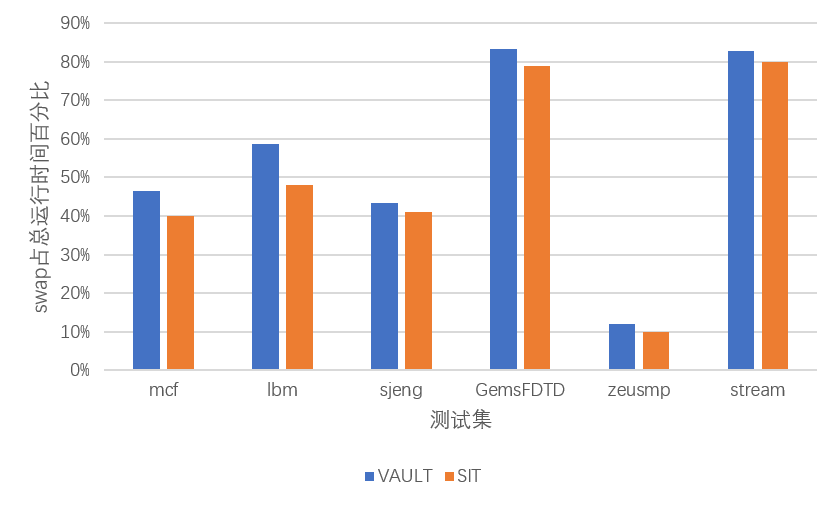
\includegraphics{eval-swap.png}
    \caption{\textbf{SPECCPU, STREAM测试集在不同完整性保护方案下swap所占比列}。}
   \label{fig:eval-swap}
\end{figure}
如图 ~\ref{fig:eval-swap}所示,我们分别测试了SIT,VAULT等先进的完整性保护方案,在超过soc上保护内存限制时候产生swap的开销占总运行时间的比例。为了能够理论上支持无限制的内存完整性保护方案,在SIT以及VAULT等方案中一旦使用的内存超过了soc可以保护的范围。CPU会选择恰当
页将其中改的数据进行加密,然后swap到非安全的内存中。为了保证从非安全内存中swap回到安全内存中,数据没有被修改。CPU在swap的时候会生成一个evict metatdate结构。该结构中记录了swap出去页的哈希值,以及属于哪一个enclave等相关的元数据,该结构被存储在安全内存中。注意当安全内存
十分紧张的时候,该数据结构也可能被swap到非安全内存中,同样我们会为存放evict metadata的页生成一个evict metadata,类似于树的形式,只需要保存根上的evict metadata既可以保证所有swap出去页的完整性。虽然SIT,vault能够理论上支持更多的内存,但是当SoC上保护得内存耗尽的时候
swap会带来很严重的性能开销,测试发现,一次swap将会带来高达40k的开销,我们在SPECCPU和STREAM测试集上进行了测试(这里我们挑选了SPECCPU中运行时内存超过128M的测试用例),我们发现swap占据了总运行时间的10\%-80\%,其中5/6的测试结果显示swap占据了总运行时间的40\%以上,其中GemsFDTD和STREAM测试swap的开销格外严重,占据了总运行时间的80\%以上,
另外杜比SIT和VAULT,在VAULT中swap的开销会更加的严重,这不是应为VAULT的设计的缺陷,还是因为VAULT运行时候的气态开销更小,导致了swap所占的时间更加明显。通过上面的数据显示,一旦使用的内存超过了SoC上保护的限制,swap将造成验证的性能降级,所以优化swap的开销非常的重要。

\begin{figure}[!htp]
    \centering
    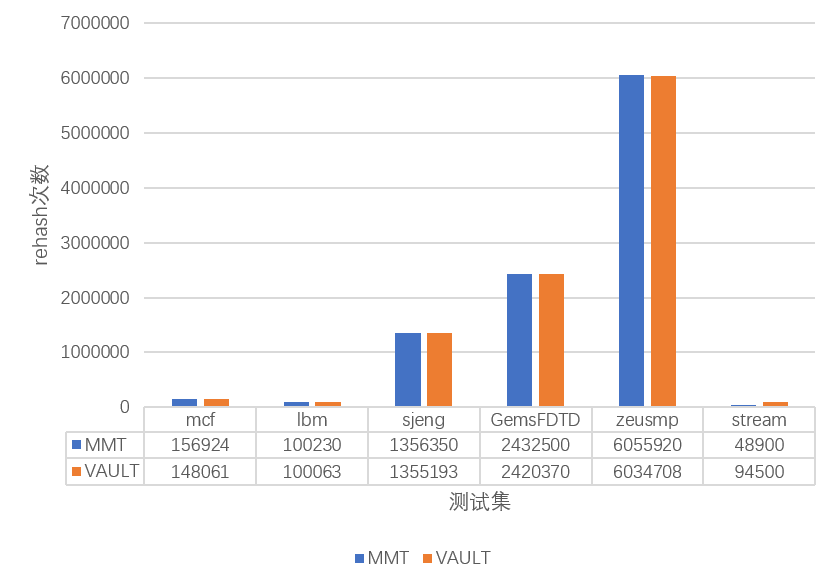
\includegraphics{eval-rehash.png}
    \caption{\textbf{SPECCPU, STREAM测试集在不同完整性保护方案下rehash的次数}。}
   \label{fig:eval-rehash}
\end{figure}
如图 ~\ref{fig:eval-rehash}所示,我们测试了VAULT和MMT中rehash的次数。为了能够增加完整性保护树中节点的扇出,VAULT和MMT都采用了分级counter的设计思路。因为分级counter会带来rehash的额外开销,来缓解replay等攻击。在MMT的设计中我们采用了三级counter的设计,三级counter的设计充分考虑了
完整性保护树中的冷热counter不均衡,在较高的树节点中往往只存在一个活跃的counter,而其他的counter可能处于不活跃的状态,所以我们可以减少冷counter比特数,增加热counter的比特数,从而兼顾安全性于节点的扇出。在这里我们同先进的VAULT完整性保护方案进行了比较。其中VAULT的稳定扇出为24,而MMT中
节点的扇出为32。在更大的扇出情况下,MMT并没造成更多的rehash的次数,说明在真实的workload下,完整性保护树中的冷热counter分布不均衡,而extra counter的设计能够很好的考虑到这种情况,从而进一步的提高树节点的扇出。在SPECCPU的测试集中,大多数的场景下,MMT于VAULT的rehash的次数相差小于1\%,
在stream的场景中,因为内存访问的比较规律,同时使用的内存较少,通过extra conter的方式能够使热counter拥有更多的比特数,从而减少热counter rehash带来的影响。所以相较于VAULT而言rehash的次数反而更少了。综上,我们认为MMT三层counter的设计充分考虑了完整性保护树的不均衡性,在实际场景中不会带来更多的
开销,在个别场景中,会比先经的VAULT的rehash开销更少。

\begin{figure}[!htp]
    \centering
    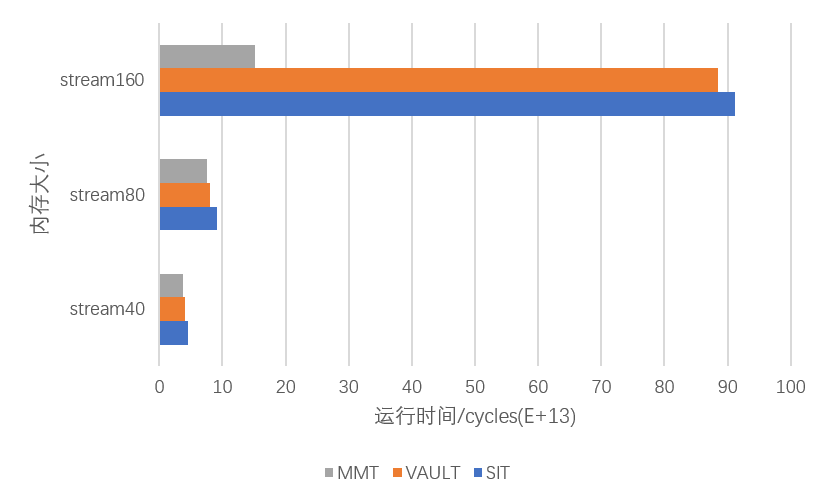
\includegraphics{eval-memorysize.png}
    \caption{\textbf{STREAM测试集使用内存大小与不同完整性保护方案下性能关系图}。}
   \label{fig:eval-memorysize}
\end{figure}
如图 ~\ref{fig:eval-memorysize}所示,我们比较程序使用不同的内存大小,对完整性检查的影响,在这里我们选取了STREAM测试集。STREAM是为了测试内存的性能的测试集,拥有较大的内存压力,频繁的读写内存能够快速耗尽SoC上能保护得安全内存得空间,同时产生频繁得swap操作。这里我们分别选取了SIT, VAULT, MMT对使用40M, 80M, 160M内存
得STREAM测试集做了分析。当程序使用的内存少于SoC上能够保护得内存时候,SIT,VAULT,MMT之间得差距并不是很明显。SIT会比MMT慢20\%左右,和VAULT相比,MMT采用了三级counter得设计,与VAULT相相比略有性能提升。因为40M和80M得内存较少,没有充分发挥三级counter得优势,当进一步扩大内存得时候三级counter得优势会更加的明显。
当使用的程序使用的内存超过了128M得时候。SIT和VAULT得性能开销急剧增加,因为STREAM会频繁循环的的访问内存,所以一旦超出了SoC上能够保护的内存时,就会频繁的发生swap操作,造成较大的性能开销。和SIT,VAULT相反,MMT采用了挂挂载的方式代替内存的swap,挂载操作的开销非常小(100~200 cycles)。所以当使用的内存扩大了一倍,
运行时间也线性的扩大了一倍,挂载操作并没有成为性能的瓶颈。而swap操作会带来7,8倍的性能开销,说明swap操作取代了完整性保护的检查,成为了主要的瓶颈。

\begin{figure}[hbt]
    \centering
    \setlength{\belowcaptionskip}{0pt}
    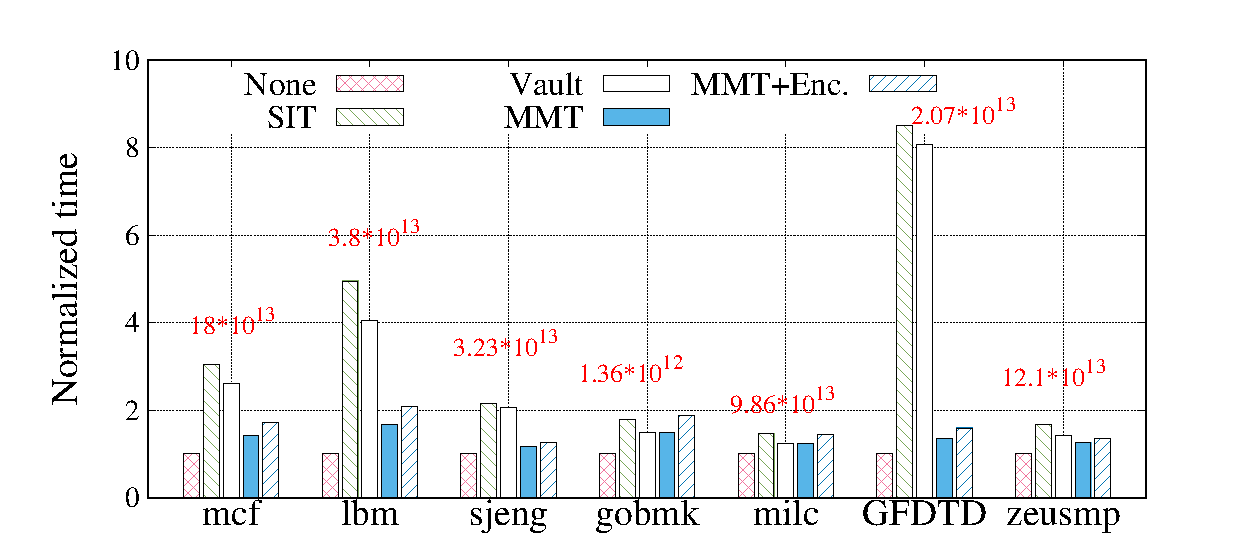
\includegraphics[scale=0.6]{fig/eval-integrity-bench.eps}
    \caption{\textbf{SPECCPU测试集在不同完整性保护方式下的性能}. \emph{None} 表示梅伊欧完整性保护下的理论性能。}
    %Compared with SGX and Vault, {\forest} can achieve the best performance in all the cases.
    \label{fig:eval-inter-bench}
\end{figure}
如图~\ref{fig:eval-inter-bench}所示,我们在SPECCPU上测试了SIT, VAULT, MMT, MMT+encrypt, 以及不做完整性检查原始的测试。其中\emph{gobmk},\emph{milc}两个测试集使用的内存小于128M,不会产生swap的开销,剩下的测试程序使用的内存从[180M:1200M]不等。从测试结果中我们可以发现,MMT的性能均优于SIT和VAULT,
在mcf的测试中,SIT和VAULT相较于没有完整性保护的程序分别会有2.05x和1.6x的开销,而MMT只有0.4x的开销,这部分的开销主要是完整性检查的开销,而挂载的开销小于1\%(挂载的操作只需要100~200的开销),在其他的测试中例如GemsFDTD,SIT和VAULT相较于不做完整性检查的程序来说有高达7.5x和7.06x倍的性能开销,而MMT只会
有0.35x的性能的开销。在这种极限的场景下,MMT相较于没有完整性保护的原程序来说只有0.35x的开销,Mount操作大幅减少了原有的swap的开销,并且在绝大多数的场景下,Mount的开销可以忽略不记(<1\%)。当使用内存小于SoC上可以保护的内存时候,MMT和Vault相比性能相近(这里为了是SoC上保护的内存相同,我们减少了MMT树的个数,因此三级counter的优势没有很好的体现)。
根据上面的测试我们可以得出,不论在内存使用超过SoC能保护的内存大小,还是小于SoC保护的内存时候,MMT都具有最好得性能,特别是当使用得内存超过SoC保护得内存大小得时候,挂载操作将极大得缓减原本swap页所带来的开销,又因为在运行时,可以通过Mount Table中读取子树的根节点来保证运行时候对完整性树检查的层数不变,从而保证SoC上内存足够的情况下,也不会带来额外的开销。


